\documentclass[a4paper, 11pt]{article}
\usepackage[english]{babel}
\usepackage{appendix}
\input{"/media/alessandro/OS/Users/ale57/Documents/1. universita'/ANNO IV (2019-2020)/second semester/header.tex"}

\begin{document}

\title{NNDL: Homework 1 \\ Supervised Deep Learning}
\author{Alessandro Lovo}
\maketitle

\section{Introduction}
  This homework consists in applying supervised deep learning to two tasks: a regression task consisting in approximating a scalar function of a scalar variable and a classification task that is recognizing the handwritten digits of the MNIST dataset. For the regression task a fully connected network (FCN) will be used, while for the classification task both a fully connected but most importantly convolutional networks (CNN) will be tested. In both cases different architectures, optimization and visualization techniques and hyperparameter search will be tried.

  \subsection{General framework}
    Both tasks rely on a framework of python classes that unfolds as follows:
    \begin{itemize}
      \item \textbf{Net}: class inheriting from \emph{torch.nn.Module} that contains the actual neural network with a specific architecture.
      \item \textbf{Evolver}: class for handling the training and validation of a \emph{Net}. In this class there is a check at the end of every training epoch to interrupt the learning process. To implement early stopping one just needs to inherit from the \emph{Evolver} class and specify that check condition. In particular the learning process stops if the validation loss isn't decreasing after \emph{patience} number of epochs.
      \item \textbf{KFoldCrossValidator}: class for performing k fold cross validation on a particular set of hyperparameters.
    \end{itemize}

\section{Regression task}
  \subsection{Basic solution}
    The data for this task consists in 100 points for training, arranged in such a way to leave two 'gaps' (fig \ref{fig:r:basic} b), and 100 test points that fill the gaps, allowing to test how good the net is in generalizing its learning.

    As a basic solution I implemented a two layered FCN with 128 neurons per hidden layer, the sigmoid as activation function and trained it for 2000 epochs using the Adam optimizer with learning rate set to $10^{-3}$ and a batch size of 10 datapoints. The loss function used is the mean square error (MSE) and 10\% of training data is used for validation. In fig \ref{fig:r:basic} are shown the results and one can see that the model is, unsurprisingly, not very good. In particular the validation loss started to increase just after 500 epochs and still there is some underfitting on the training data.
    To solve these issues one requires both a more complex model and some regularization techniques.

    \begin{figure}
      \centering
      \subfloat[]{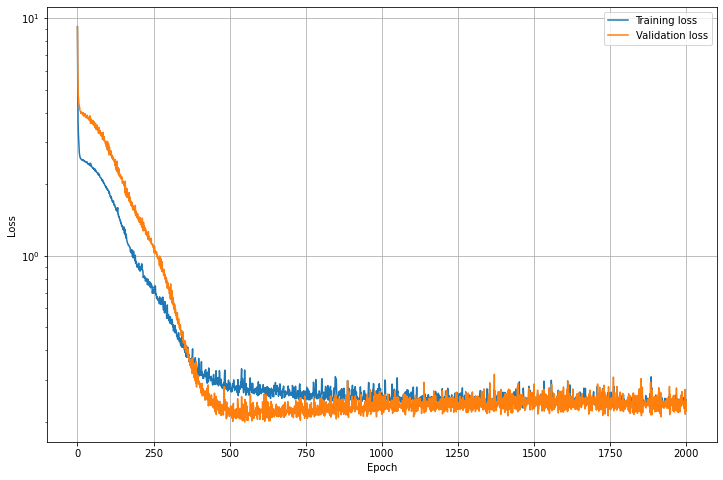
\includegraphics[width=0.45\textwidth]{img/regression/basic_loss.png}} \quad
      \subfloat[]{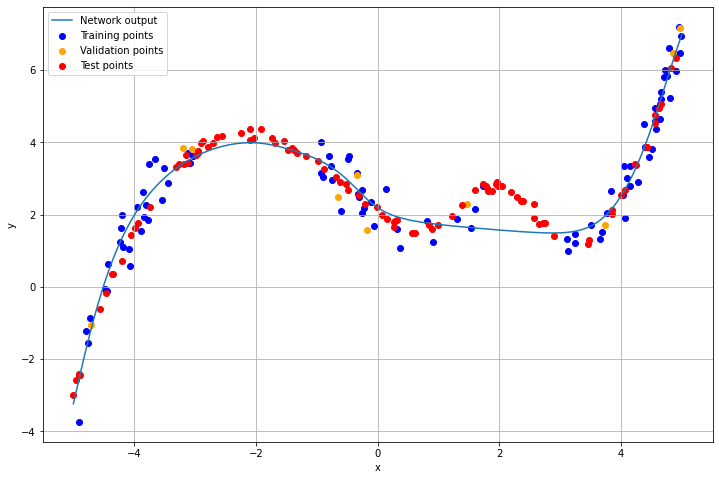
\includegraphics[width=0.45\textwidth]{img/regression/basic_plot.png}}
      \caption{Results of the basic solution: training and validation loss as a function of epoch number (a) and Output of the trained network compared with training, validation and test datapoints (b).}
      \label{fig:r:basic}
    \end{figure}

  \subsection{More advanced methods}
    Since there is quite few training data, the result is highly dependent on the train-validation split, so to improve this, in the following, every set of hyperparameters will be tested with a 5-fold setup.
    Also it is worth introducing the early stopping in order to be able to increase the maximum number of epochs (for example up to $10^4$) without worrying about overfitting. In practice this is implemented creating a checkpoint for the network every time the validation loss reaches a new minimum; if there is no new minimum after \emph{patience} epochs, learning stops and the net is reverted back to the last checkpoint.
    At this point one can test different architectures (2, 3 or 4 layers with or without dropout and different activation functions: Sigmoid, ReLU or Tanh) and optimization procedure (momentum for the SGD optimizer and weight decay for the Adam optimizer).

    Since the number of combinations of hyperparameters rockets, it would be better to rule out some of these possibilities.
    In particular Adam yields reliably better results than SGD with momentum, and also the Sigmoid activation function frequently causes a substantial underfitting. Also having a too small training batch size makes the learning process very unstable and on average a 4-layered network performs better than a 3-layered one. So, the architecture to be tested now is a network with 4 hidden linear layers, where the second and third one are followed by a dropout layer.

    At this points the remaining degrees of freedom are the following, and for each of them I provided a list of possibilities to be tested in a random search
    \begin{itemize}
      \item the number of neurons in each layer: [8, 16, 32, 64, 128, 256]
      \item dropout probabilities: [0, 0.15, 0.35, 0.5]
      \item activation function: [Tanh, ReLU]
      \item learning rate and weight decay for the Adam optimizer: respectively [$10^{-4}$, $5\cdot10^{-4}$, 0.001, 0.005, 0.01, 0.05] and [0, $10^{-5}$, $5\cdot10^{-5}$, $10^{-4}$, $5\cdot10^{-4}$, 0.001]
      \item patience parameter for the early stopping: [100, 200, 300, 400]
      \item training batch size: [20, 30, 40, 50]
    \end{itemize}
    To speed up the random search I also implemented trial pruning, i.e., if in one of the first three folds the validation loss is above 0.4, the remaining folds are not computed, directly testing the next hyperparameter combination and thus saving time.

  \subsection{Results}
    After 65 non pruned iterations of the random search the best hyperparameter combination is found in hidden layers with 32, 128, 64, 256 neurons, with 0.5 dropout probability after the second layer and Tanh as activation function, trained with learning rate of 0.001, no weight decay, a train batch size of 30 and patience of 400, resulting in an average validation loss of 0.227.
    Since during the random search networks weren't saved, now I performed a final 5-fold run with the best hyperparameters and selected the best of the five nets obtaining the results in fig \ref{fig:r:best}. If one compares with the basic, solution this one doesn't seem much better, however by comparing the two test losses, the best net performs quite better, proving to be more able to generalize than the basic one (tab \ref{tab:r:losses}).

    If one visualizes the weight histogram of the weights can see that, due to the lack of weight decay, the weights are not very peaked around 0, and also the distribution is broader on the second layer, where dropout was applied. On the other hand the activation profiles are not very interpretable (fig \ref{fig:r:visualization}).

    \begin{figure}
      \centering
      \subfloat[]{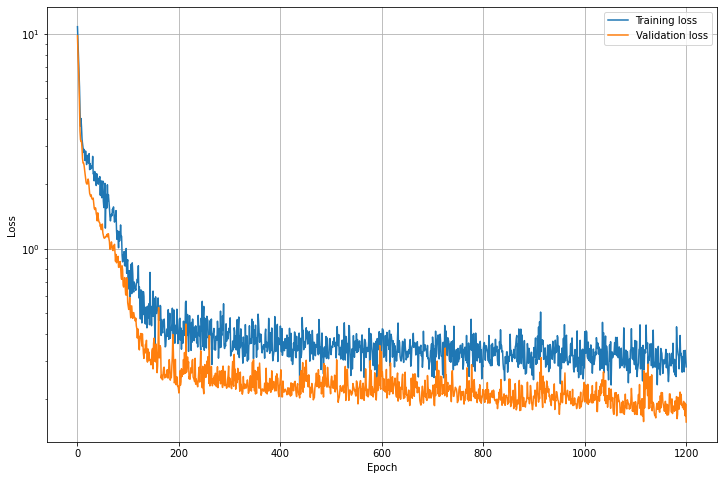
\includegraphics[width=0.45\textwidth]{img/regression/best_loss.png}} \quad
      \subfloat[]{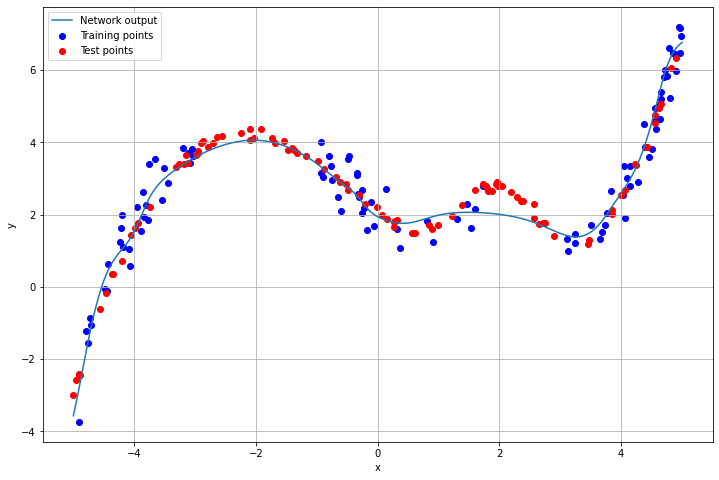
\includegraphics[width=0.45\textwidth]{img/regression/best_plot.png}}
      \caption{Results of the best network: training and validation loss as a function of epoch number (a) and Output of the trained network compared with training/validation in blue and test datapoints in red (b).}
      \label{fig:r:best}
    \end{figure}

    \begin{table}
      \centering
      \begin{tabular}{c|ccc}
        Net & Training loss & Validation loss & Test loss \\
        \midrule
        Basic & 0.2418 & 0.2375 & 0.3417 \\
        Best & 0.3008 & 0.1822 & 0.1216
      \end{tabular}
      \caption{Comparison of the losses of the basic and best net.}
      \label{tab:r:losses}
    \end{table}

    \begin{figure}[H]
      \centering
      \subfloat[]{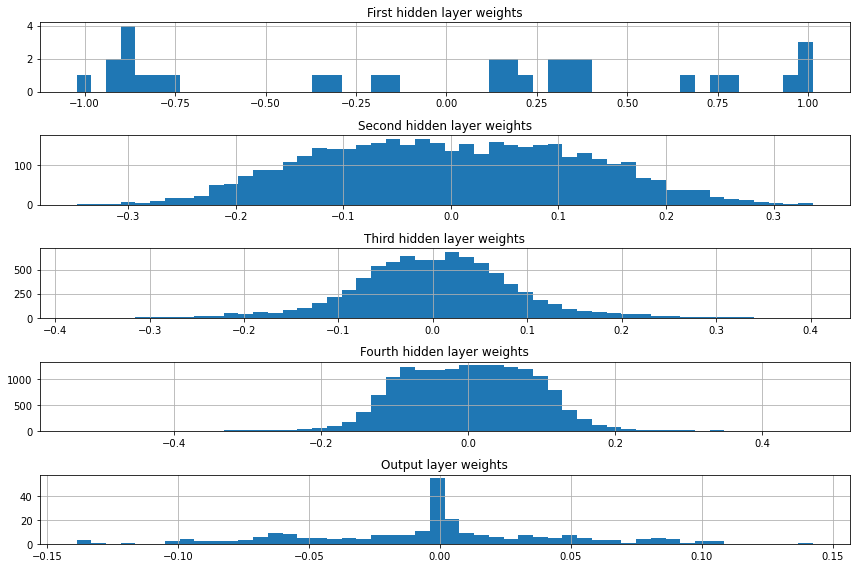
\includegraphics[width=0.45\textwidth]{img/regression/best_w.png}} \quad
      \subfloat[]{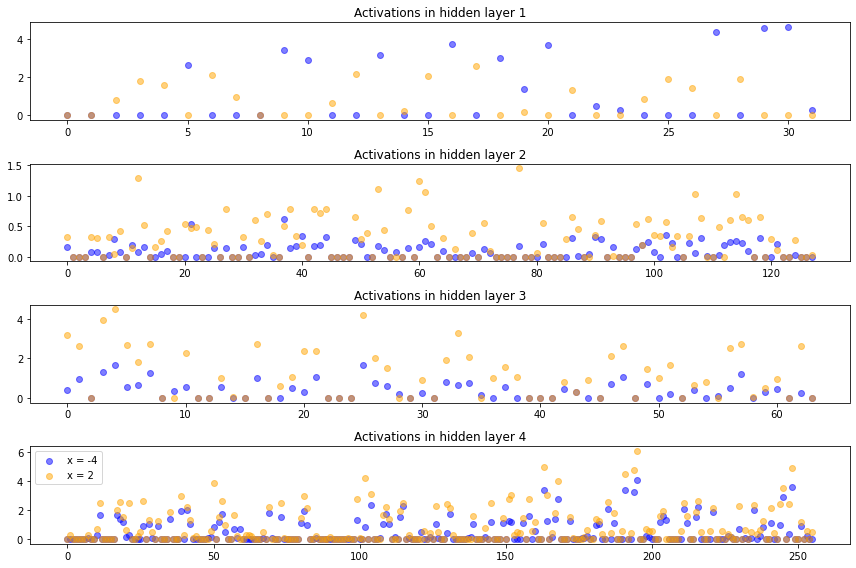
\includegraphics[width=0.45\textwidth]{img/regression/best_act.png}}
      \caption{Visualization of the weights and activations of the best net when provided two different inputs: $x = -4$ and $x = 2$.}
      \label{fig:r:visualization}
    \end{figure}


\section{Classification task}
  \subsection{Methods}
    For this task the data consists in 28 by 28 pixels gray scale images of handwritten digits: 60000 for training and validation and 10000 for testing. Since there is a lot of data and the learning process takes quite a lot of time I used cross validation only for hyperparameter optimization, while manually testing different architectures is performed using the same 20\% of the training data as validation for all of them.
    For all nets I used the \emph{CrossEntropyLoss} and ReLU as activation function, learning with the Adam optimizer, a batch size of 256 and early stopping with \emph{patience} of 10 epochs.
    The architectures I tested manually are:

    \begin{itemize}
      \item [FCN] Network with two hidden linear layers with 128 and 16 neurons trained with learning rate $10^{-3}$
      \item [CNN] Network with three convolutional layers with channels [8, 16, 32], kernel size of 3, stride of 2, paddding of 1 in the first two layers and 0 for the last one. Then, after the convolutonal part, two linear layers with 128 and 16 neurons. The net is trained with learning rate $10^{-3}$ and weight decay of $10^{-4}$
      \item [DCNN] Network with the same structure as the previous one but introducing two dropout layers before the linear layers, each one with dropout probability of 0.5
      \item [PDCNN] Same network as the DCNN but with 11 neurons on the output layer, thus adding a class for 'not a number'. This net is trained with the regular MNIST data plus images with Perlin noise and a label equal to 10. In practice this is achieved modifying the \emph{transform} attribute of the training dataset in such a way that with probability 0.09 instead of providing a MNIST image, it generates Perlin noise.
    \end{itemize}

    At every increase in complexity the validation loss kept decreasing (tab \ref{tab:c:losses}), however the last architecture proved much slower to train due to the generation of noise images, so the maximum complexity tested in hyperparameter optimization was the one of the DCNN. Also to better evaluate every combination of hyperparameters, I proceeded with a 5-fold setup, but, for time reasons, running only the first two folds. Basically this is similar to performing twice a 80\%-20\% training-validation random split. Also I added to the validation loss a penalty equal to $10^{-5}$ times the training time in minutes, in order to privilege a simpler architecture in case of similar performances.

    The hyperparameter optimization was performed with \emph{optuna} at its default settings on the following degrees of freedom:

    \begin{itemize}
      \item Number of convolutional layers: 2, 3 or 4
      \item Number of channels: from 4 to $4\cdot2^j$ for the $j^{th}$ convolutional layer
      \item Kernel size: from 2 to 6. Stride: from 1 to 4. Padding: 0 or 1
      \item Dropout probability: from 0 to 0.7
      \item Number of neurons in the linear layers: from 16 to 256 for the first one and from 4 to 128 for the second one
      \item Learning rate: from $10^{-5}$ to $10^{-1}$. Weight decay: from $10^{-7}$ to $10^{-1}$
    \end{itemize}
    One has to notice that some sets of hyperparameters yield an invalid network, for example if the strides are too large and so no pixel survives: in this case the trial is simply pruned. However, since the more convoulutional layers, the higher the probability that this happens, in the end there were no valid four layered networks in the study.

  \subsection{Results}
    The optimization ran for 50 trials, 28 of which were pruned due to an invalid architecture. A visualization of the optuna study can be seen in appendix \ref{app:optuna}. The best combination of hyperparamers is a network with 3 convolutional layers with channels [4, 15, 19], kernel sizes [3, 3, 4], strides [3, 1, 2] and paddings [0, 1, 1]; dropout probabilities [0.4726, 0.6960] and linear layers with [129, 69] neurons; trained with learning rate of $9.485\cdot10^{-4}$ and weight decay of $9.392\cdot10^{-6}$.

    In tab \ref{tab:c:losses} are reported the performances of the different architectures, where the test accuracy is computed as the fraction of correctly classified samples considering the net's choice as the class with the higher output value. It is important to observe that the test accuracy was not a criterion for choosing the net architecture or tuning hyperparameters: it is just a way to evaluate the different models in the end with something more intuitive than the value of the \emph{CrossEntropyLoss}.

    Also another interesting alternative to evaluate the best net performance is trying to feed it Perlin noise and see its output. As one can see from fig \ref{fig:c:ptest} the net is pretty puzzled by the perlin noise (b), however, curiously, when it thinks it is seeing a number, it thinks of an 8 (c). Anyways even in this case the net output is far from being as sharp as when provided a real number (a), and this is a symptom that the training worked properly.

    \begin{figure}
      \centering
      \subfloat[]{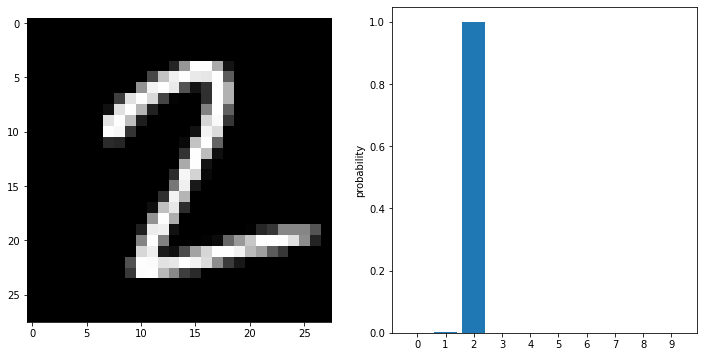
\includegraphics[width=0.31\textwidth]{img/classification/test2.png}} \,
      \subfloat[]{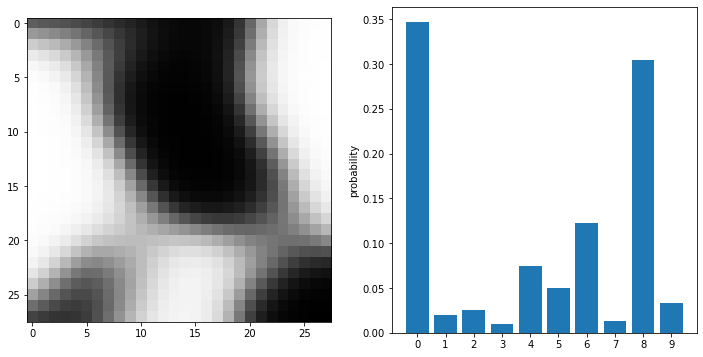
\includegraphics[width=0.31\textwidth]{img/classification/perlin_test1.png}} \,
      \subfloat[]{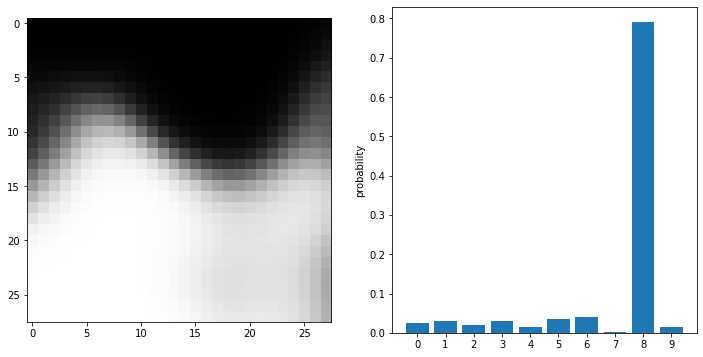
\includegraphics[width=0.31\textwidth]{img/classification/perlin_test2.png}}
      \caption{Probability of each class provided the input image shown. In the first image the net is given a MNIST test sample, while in the other two Perlin noise.}
      \label{fig:c:ptest}
    \end{figure}

    To better understand what the nets are doing one can optimize an input image to maximize the activation of a specific neuron. In fig \ref{fig:c:act} are the results of this optimization for the output neurons of different networks. The optimization is achieved starting from a gray image (all pixels set to 0.5) and using the Adam optimizer with learning rate 0.1 and weight decay 0.01. Also, in order to avoid the simple increasing of the contrast of the image (pixel values above 1 or below 0), the image passes through a sigmoid before being fed to the net.

    Other visualization techniques are plotting the weights of the first hidden layer for the FCN, where one can see the development of some edge detectors, and the feature space analysis for the CNN, which is however a bit harder to interpret (appendix \ref{app:visualization})

    \begin{table}[H]
      \centering
      \begin{tabular}{c|ccc}
        Net & training loss & validation loss & test accuracy \\
        \midrule
        FCN & 0.0138 & 0.1087 & 0.9735 \\
        CNN & 0.0308 & 0.0762 & 0.9819 \\
        DCNN & 0.0819 & 0.0463 & 0.9887 \\
        PDCNN & 0.0580 & 0.0421 & 0.9898 \\
        \midrule
        best & 0.1062 & 0.0527 & 0.9873
      \end{tabular}
      \caption{Performance of the manually tested net and the best one from optuna optimization.}
      \label{tab:c:losses}
    \end{table}

    \begin{figure}[H]
      \centering
      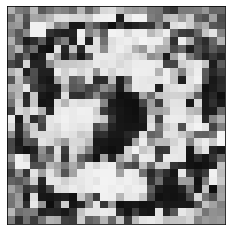
\includegraphics[width=0.09\textwidth]{img/classification/FCN_b0.png}
      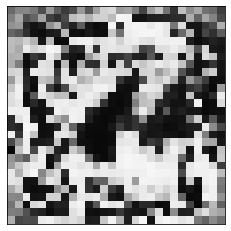
\includegraphics[width=0.09\textwidth]{img/classification/FCN_b1.png}
      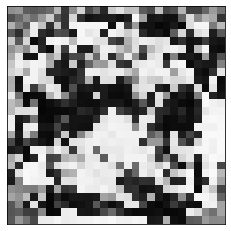
\includegraphics[width=0.09\textwidth]{img/classification/FCN_b2.png}
      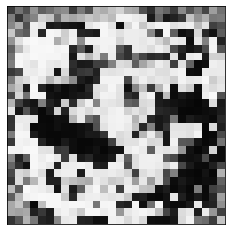
\includegraphics[width=0.09\textwidth]{img/classification/FCN_b3.png}
      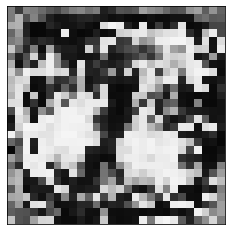
\includegraphics[width=0.09\textwidth]{img/classification/FCN_b4.png}
      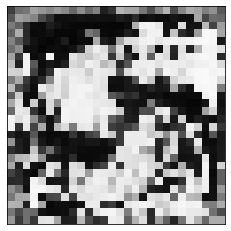
\includegraphics[width=0.09\textwidth]{img/classification/FCN_b5.png}
      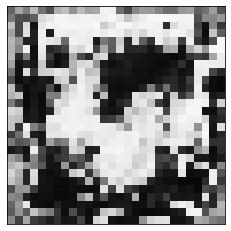
\includegraphics[width=0.09\textwidth]{img/classification/FCN_b6.png}
      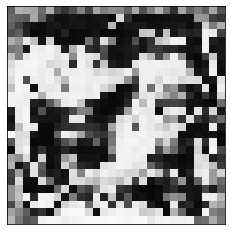
\includegraphics[width=0.09\textwidth]{img/classification/FCN_b7.png}
      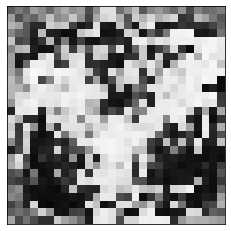
\includegraphics[width=0.09\textwidth]{img/classification/FCN_b8.png}
      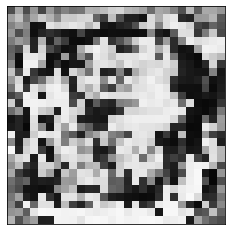
\includegraphics[width=0.09\textwidth]{img/classification/FCN_b9.png}

      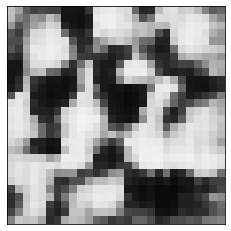
\includegraphics[width=0.09\textwidth]{img/classification/CNN_b0.png}
      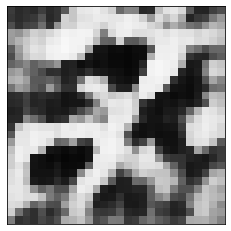
\includegraphics[width=0.09\textwidth]{img/classification/CNN_b1.png}
      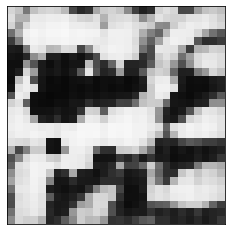
\includegraphics[width=0.09\textwidth]{img/classification/CNN_b2.png}
      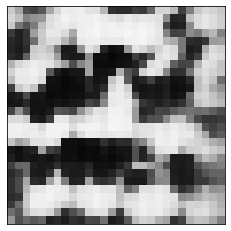
\includegraphics[width=0.09\textwidth]{img/classification/CNN_b3.png}
      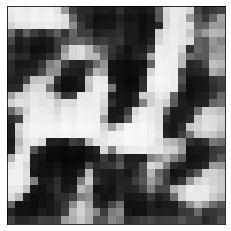
\includegraphics[width=0.09\textwidth]{img/classification/CNN_b4.png}
      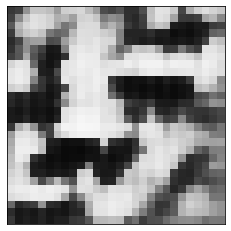
\includegraphics[width=0.09\textwidth]{img/classification/CNN_b5.png}
      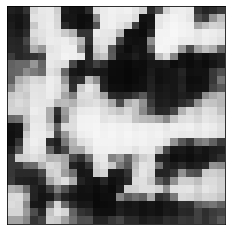
\includegraphics[width=0.09\textwidth]{img/classification/CNN_b6.png}
      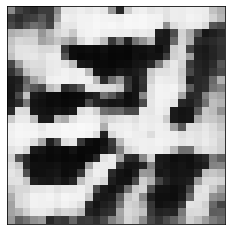
\includegraphics[width=0.09\textwidth]{img/classification/CNN_b7.png}
      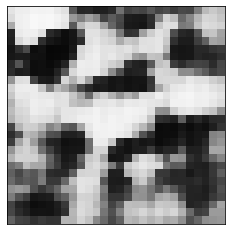
\includegraphics[width=0.09\textwidth]{img/classification/CNN_b8.png}
      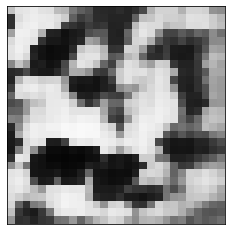
\includegraphics[width=0.09\textwidth]{img/classification/CNN_b9.png}

      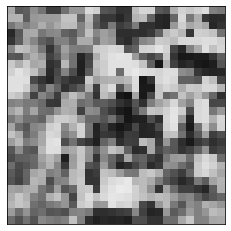
\includegraphics[width=0.09\textwidth]{img/classification/DCNN_b0.png}
      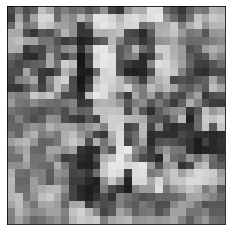
\includegraphics[width=0.09\textwidth]{img/classification/DCNN_b1.png}
      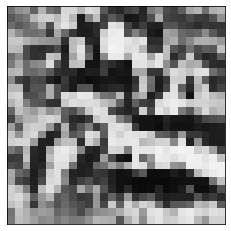
\includegraphics[width=0.09\textwidth]{img/classification/DCNN_b2.png}
      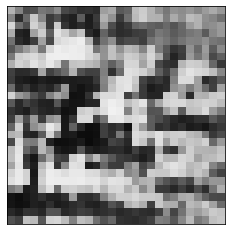
\includegraphics[width=0.09\textwidth]{img/classification/DCNN_b3.png}
      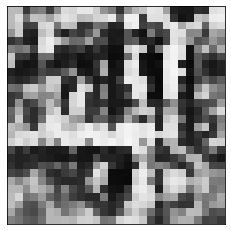
\includegraphics[width=0.09\textwidth]{img/classification/DCNN_b4.png}
      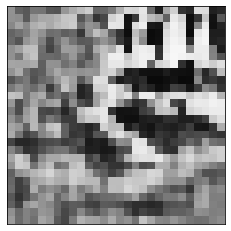
\includegraphics[width=0.09\textwidth]{img/classification/DCNN_b5.png}
      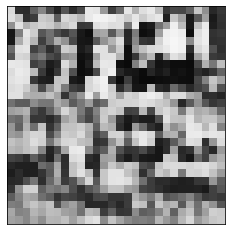
\includegraphics[width=0.09\textwidth]{img/classification/DCNN_b6.png}
      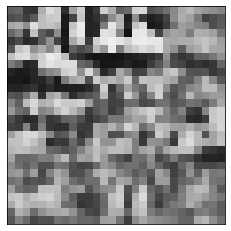
\includegraphics[width=0.09\textwidth]{img/classification/DCNN_b7.png}
      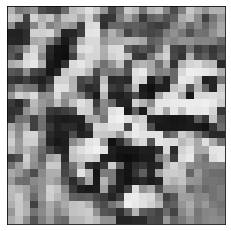
\includegraphics[width=0.09\textwidth]{img/classification/DCNN_b8.png}
      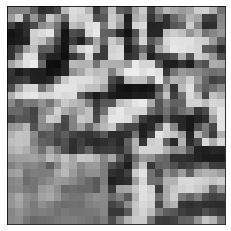
\includegraphics[width=0.09\textwidth]{img/classification/DCNN_b9.png}

      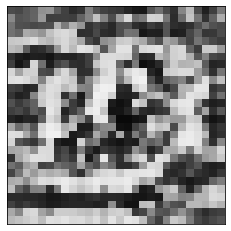
\includegraphics[width=0.09\textwidth]{img/classification/PDCNN_b0.png}
      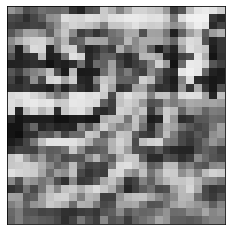
\includegraphics[width=0.09\textwidth]{img/classification/PDCNN_b1.png}
      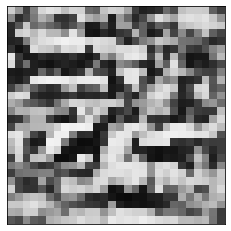
\includegraphics[width=0.09\textwidth]{img/classification/PDCNN_b2.png}
      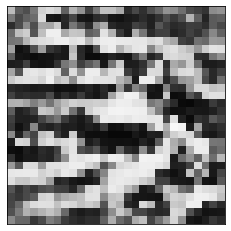
\includegraphics[width=0.09\textwidth]{img/classification/PDCNN_b3.png}
      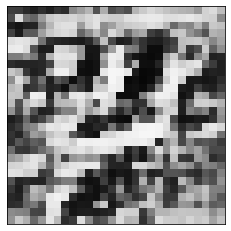
\includegraphics[width=0.09\textwidth]{img/classification/PDCNN_b4.png}
      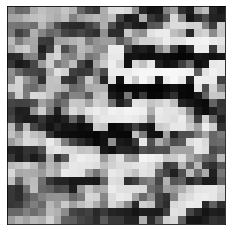
\includegraphics[width=0.09\textwidth]{img/classification/PDCNN_b5.png}
      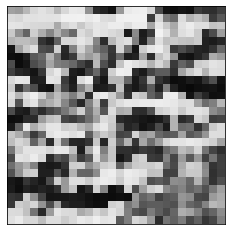
\includegraphics[width=0.09\textwidth]{img/classification/PDCNN_b6.png}
      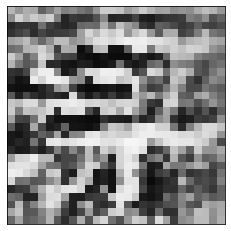
\includegraphics[width=0.09\textwidth]{img/classification/PDCNN_b7.png}
      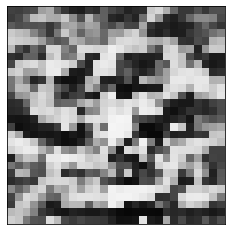
\includegraphics[width=0.09\textwidth]{img/classification/PDCNN_b8.png}
      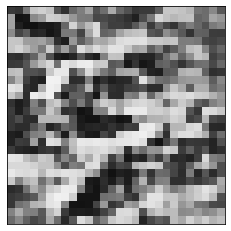
\includegraphics[width=0.09\textwidth]{img/classification/PDCNN_b9.png}
      % 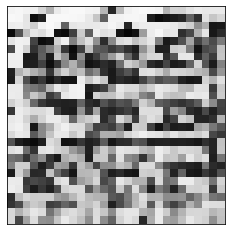
\includegraphics[width=0.09\textwidth]{img/classification/PDCNN_bn.png}

      \includegraphics[width=0.09\textwidth]{img/classification/BN_b0.png}
      \includegraphics[width=0.09\textwidth]{img/classification/BN_b1.png}
      \includegraphics[width=0.09\textwidth]{img/classification/BN_b2.png}
      \includegraphics[width=0.09\textwidth]{img/classification/BN_b3.png}
      \includegraphics[width=0.09\textwidth]{img/classification/BN_b4.png}
      \includegraphics[width=0.09\textwidth]{img/classification/BN_b5.png}
      \includegraphics[width=0.09\textwidth]{img/classification/BN_b6.png}
      \includegraphics[width=0.09\textwidth]{img/classification/BN_b7.png}
      \includegraphics[width=0.09\textwidth]{img/classification/BN_b8.png}
      \includegraphics[width=0.09\textwidth]{img/classification/BN_b9.png}

      \caption{Input images that maximize the activation of the 10 output neurons of the tested nets: from top to bottom FCN, CNN, DCNN, PDCNN, best. The FCN and best images are the ones that resemble more the digits they are supposed to represent.}
      \label{fig:c:act}
    \end{figure}



\newpage
\begin{appendices}
  \section{Tables and plots of the hyperparameter optimization} \label{app:optuna}
    For the random search of the regression task see \url{code/regression/random_search5.csv}.

    For the search with optuna see \url{code/classification/optuna_search3.csv}. Moreover from the colab notebook it is possible to load the optuna study \url{code/classification/optuna_search3.db} and view it in its entirety. In fig \ref{fig:c:optuna}  are some example plots of that study.

    \begin{figure}[H]
      \centering
      \includegraphics[width=0.27\textwidth]{img/classification/o_ch1-ch2.png}
      \includegraphics[width=0.27\textwidth]{img/classification/o_Nh1-Nh2.png}
      \includegraphics[width=0.27\textwidth]{img/classification/o_lr-wd.png}
      \includegraphics[width=0.9\textwidth]{img/classification/o_importance.png}
      \caption{(Top): Contour plots of, respectively: the number of channels in the first two convolutional layers; the number of neurons in the two hidden linear layers; learning rate and weight decay. (Bottom): Importance of the different hyperparameters (\emph{ks*} is the kernel size of convolutional layer * and \emph{ch*} is its number of channels; \emph{p*} is the dropout probability applied before the linear layer *; \emph{ncl} is the number of convolutional layers; other hyperparameter names are self explanatory.)}
      \label{fig:c:optuna}
    \end{figure}


  \section{Further visualization techniques for the classification task} \label{app:visualization}
    \begin{figure}[H]
      \centering
      \includegraphics[width=0.25\textwidth]{img/classification/CNN_fs1.png}
      \includegraphics[width=0.3\textwidth]{img/classification/CNN_fs2.png}
      \includegraphics[width=0.25\textwidth]{img/classification/CNN_fs3.png}
      \caption{Feature space analysis of the CNN}
      \label{fig:c:CNN_fs}
    \end{figure}

    \begin{figure}[H]
      \centering
      \includegraphics[width=0.7\textwidth]{img/classification/FCN_weights.png}
      \caption{Plot of the weights of the first hidden layer of the FCN}
      \label{fig:c:FCN_w}
    \end{figure}

\end{appendices}

\end{document}
